% pgfplots-lines.tex — publication line plot template (standalone).
% For small or symbolic data. Large experiment CSVs belong to matplotlib
% (see figure-matplotlib skill).
% Compile with latex-compile-standalone; PDF lands next to this file.
\documentclass[tikz,border=4pt]{standalone}
\usepackage{pgfplots}
\pgfplotsset{compat=1.18}

% Okabe-Ito colorblind-safe cycle (matches figure-matplotlib).
\definecolor{oiblue}{HTML}{0072B2}
\definecolor{oiorange}{HTML}{E69F00}
\definecolor{oigreen}{HTML}{009E73}

\pgfplotsset{
  pub/.style={
    width=8.6cm, height=5.4cm,       % single-column friendly
    font=\small,
    xlabel={Training step},
    ylabel={Validation loss},
    grid=both, grid style={black!10},
    axis line style={black!60},
    legend style={draw=none, fill=none, font=\footnotesize},
    legend cell align=left,
  },
}

\begin{document}
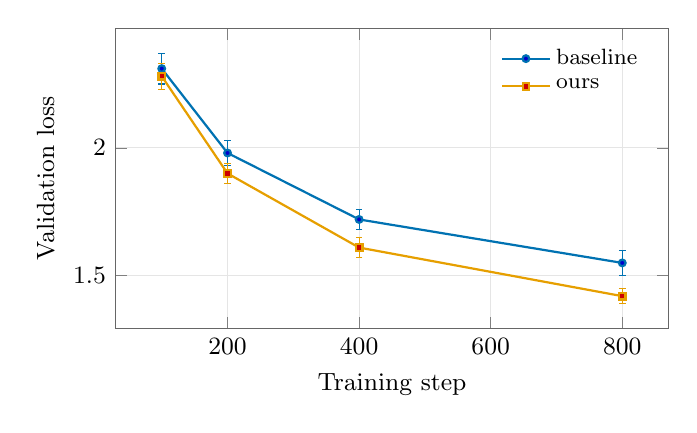
\begin{tikzpicture}
\begin{axis}[pub, legend pos=north east]

% series 1: inline coordinates (fine for small data)
\addplot+[color=oiblue, thick, mark=*, mark size=1.2pt,
          error bars/.cd, y dir=both, y explicit]
  coordinates {
    (100, 2.31) +- (0, 0.06)
    (200, 1.98) +- (0, 0.05)
    (400, 1.72) +- (0, 0.04)
    (800, 1.55) +- (0, 0.05)
  };
\addlegendentry{baseline}

% series 2: from table data (x=step, y=loss, y error=err)
\addplot+[color=oiorange, thick, mark=square*, mark size=1.2pt,
          error bars/.cd, y dir=both, y explicit]
  table[x=step, y=loss, y error=err] {
  step  loss  err
  100   2.28  0.05
  200   1.90  0.04
  400   1.61  0.04
  800   1.42  0.03
  };
\addlegendentry{ours}

\end{axis}
\end{tikzpicture}
\end{document}
